\chapter{Atividades de Observação} % (fold)
\label{chap:Atividades de Observação}
É recomendado aos estagiários de Licenciatura que reservem uma parte de suas cargas horárias de estágio, para atividades de observação de aulas e reuniões pedagógicas, o resultados destas observações é descrito neste Capítulo, em que observou-se algumas aulas do professor regente e um Conselho de Classe. Estas atividades foram desenvolvidas em grande parte para conhecer um pouco melhor sobre a turma de aplicação das regências a 2ª Série do \ac{NEM}.

\section{Análises das Aulas Observadas} % (fold)
\label{sub:Análises das Aulas Observadas}
\setlength\intextsep{0pt}
\begin{wraptable}{r}{9cm}
	\centering
	\resizebox{\linewidth}{!}{%
		\begin{tabular}{|r|c|l|}
			\hline
			\multicolumn{1}{|c|}{\textbf{Data}} & \textbf{Turma} & \multicolumn{1}{c|}{\textbf{Assunto}} \\ \hline
			\textbf{22/03} & \textbf{3(4)} & Lei de Coulomb (Exercícios)                  \\ \hline
			\textbf{}      & \textbf{2(6)} & Calorimetria (Exercícios)                    \\ \hline
			\textbf{}      & \textbf{2(6)} & Calorimetria (Revisão)                       \\ \hline
			\textbf{24/03} & \textbf{3(4)} & Corrente Elétrica (Introdução)               \\ \hline
			\textbf{}      & \textbf{2(6)} & Calorimetria (Avaliação)                     \\ \hline
			\textbf{}      & \textbf{2(6)} & Calorimetria (Correção)                      \\ \hline
			\textbf{31/03} & \textbf{1(5)} & Movimento Retilíneo Uniforme (Introdução)    \\ \hline
			\textbf{}      & \textbf{2(6)} & Dilatação Térmica (Exp. Demostrativo)        \\ \hline
			\textbf{05/05} & \textbf{3(4)} & Corrente Elétrica (Revisão)                  \\ \hline
			\textbf{}      & \textbf{1(5)} & Vetores (Introdução)                         \\ \hline
		\end{tabular}%
	}
	\caption{Acompanhamento de aulas}
	\label{tab:acompanhamento-aulas}
\end{wraptable}
Um total de 14 aulas foram observadas em dias distintos, das quais selecionou-se 10 para análise das abordagens e metodologias utilizadas pelo professor supervisor no decorrer de aplicação do programa (\textit{v. capítulo anterior}). A \autoref{tab:acompanhamento-aulas} resume as turmas, datas e assuntos de cada aula observada. Apenas para não extender-se exautivamente nestas análises, agrupou-se convenientemente as abordagens utilizadas pelo supervisor e submeteu-se às análises, ficando assim classificadas: 1) abordagens de introdução de conteúdo; 2) abordagens experimentais e 3) abordagens de exercícios e/ou revisão.

\subsection{Abordagens de Introdução de Conteúdo} % (fold)
\label{sub:Abordagens de Introdução de Conteúdo}
Ao preceder à um novo conteúdo, foram sempre observados nas aulas do professor supervisor, momentos em que a conceituação parte de situações próximas ao cotidiano do aluno, como por exemplo: na aula de introdução à análise vetorial (aula 05/05) o professor teve por pretenção construir o conceito de \textit{vetor resultante}, e o fez a partir de uma situação em que "um automóvel quebrado é preciso ser conduzido até à oficina mecânica empurrado"~, com este simples exemplo, revisou com os estudantes em tom de diálogo e descontração, as principais propriedades de uma grandeza vetorial como intensidade, direção e sentido, a partir de então sugeriu:

\begin{center}
	\begin{minipage}{.9\textwidth}
		\begin{itemize}
			\item [\textbf{Prof.:}] Ta, nós acabamos de ver que três pessoas empurrando o carro juntos e na mesma direção é melhor do que duas, que é melhor do que uma, certo?!
			\item [\textbf{Alunos:}] ...\textit{-- Todos concordaram!}
			\item [\textbf{Prof.:}] Agora imaginem uma pessoa bem forte, dessas que praticam academia 
			\item [\textbf{A1:}] Um maromba, sôr
			\item [\textbf{Prof.:}] Isso! Pode ser
		\end{itemize}			
	\end{minipage}	
\end{center}

\begin{center}
	\begin{minipage}{.9\textwidth}
		\begin{itemize}
			\item [\textbf{Prof.:}] Pessoal, o que significa eu substituir uma pessoa com o triplo de força de uma pessoa normal \textit{-- Aponta para o esquema de um "maromba"~feito no quadro}, por estas três pessoas aqui? \textit{-- Aponta para o esquema representativo de três pessoas feitas em "zé palitos"~no quadro.}
			\item [\textbf{A1:}] Nada...
			\item [\textbf{A2:}] Da na mesma né professor
			\item [\textbf{Prof.:}] Por que da na mesma?
			\item [\textbf{Vários:}] [...] É que é igual,... Os três juntos vão fazer a mesma coisa que só o fortão já da conta...
			\item [\textbf{Prof.:}] Exatamente! Isso é o que a gente vai chamar a partir de agora de Vetor Resultante. \textit{-- Segue com as explicações}
		\end{itemize}
	\end{minipage}		
\end{center}
Práticas como estas são altamente recomendáveis, o que segundo indica \citeonline{CARVALHO:1999}, o docente busca estrategicamente aproximar os conceitos relativos da unidade de ensino em estudo, ao universo sensível do estudante, o que efetivamente é capaz de promover uma passagem tênue da linguagem coloquial para a científica de forma natural.

As diversas formas da \textit{abordagem comunicativa} também se fez presente nestas situações, tal como relatam \citeonline{MORTIMER2002} na pesquisa, o professor utiliza significativamente os padrões de interações verbais e a medida que as discussões são alimentadas as tríades I-R-A vão dando lugares às tríades I-R-F-R-[...]\footnote{Atividades discursivas em salas de aulas, são capazes de gerar padrões de interações verbais do tipo: (I) Indagação do professor; (R) Resposta do aluno; (A) Avaliação do professor e (F) Feedback do aluno.} formando padrões de interações cada vez mais complexos, qualificando assim o debate.


% subsection Abordagens de Introdução de Conteúdo (end)
\subsection{Abordagens Experimentais} % (fold)
\label{sub:Abordagens Experimentais}
A atividade experimental observada, foi realizada na aula do dia 31/03 na turma 2(6), nesta ocasião o professor supervisor utilizou um aparato experimental constuído por ele próprio, uma foto do aparato pode ser vista na \autoref{fig:exp-aparato}.

O experimento consiste numa barra de cobre que quando aquecida, faz deslocar-se horizontalmente um ponteiro por efeito de dilatação térmica, este por sua vez fecha um circuíto composto por um led, o qual é aceso quando a barra atinge um dado valor de dilatação, o mesmo ocorre se a barra for resfriada e contraída até um certo valor, acendendo um outro led localizado na extremidade oposta ao primeiro e de cor diferente.

\setlength\intextsep{0pt}
\begin{wrapfigure}[10]{r}{0.5\textwidth}
	\centering
	\caption{Aparato experimental (diatação térmica)}
	\label{fig:exp-aparato}
	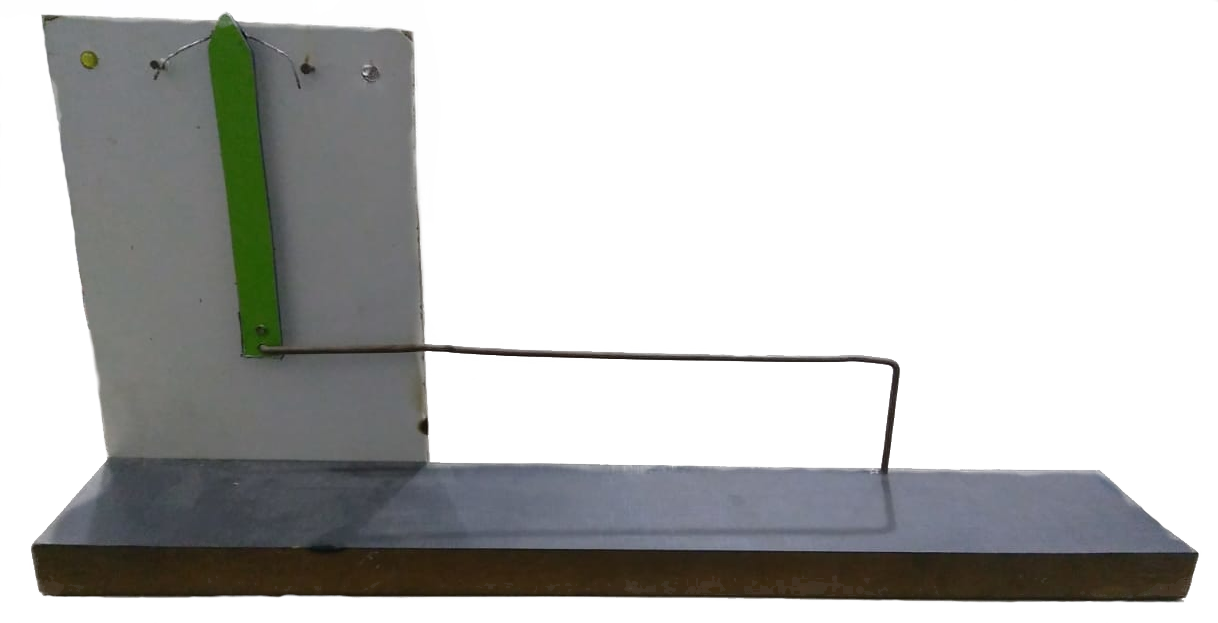
\includegraphics[width=.45\textwidth]{assets/aparato_exp.png}
	\legend{Fonte: O autor}
\end{wrapfigure}

O experimento foi conduzido de forma demostrativa, o professor após explicar a estrutura do aparato, sem revelar a termodinâmica por traz da experiência que será conduzida, questionou aos alunos de que forma poder-se-ia acender a lâmpada led sem que se toque a barra de cobre. Dessa forma desafia os alunos instigando-lhes à curiosidade e oportunizando a participação na construção do conhecimento, \citeonline[pp.~46]{CARVALHO:1999} ressalta que tal conduta é capaz de levar ao aluno perceber o conhecimento científico como um processo de construção dinâmico e aberto, favorecendo ainda mais todo o processo.
% subsection Abordagens Experimentais (end)

\subsection{Abordagens de Exercícios} % (fold)
\label{sub:Abordagens de Exercícios}
O docente utiliza estas aulas para desenvolver a dimensão do conhecimento relacionada ao Domínio Conceitual. Os exercícios propostos são em poucos números, numa lista encontram-se no máximo um total de cinco exercícios.

Em geral são exercícios fechados e de aplicação direta o que, segundo as pesquisas, se não usados corretamente permite pouca ou nenhuma mudança conceitual no aluno \cite{CLEMENT:2012}, porém quando aliados à outras abordagens de forma complementar as demais Dimensões do Conteúdo previamente trabalhados em outros momentos, pode constribuir significativamente para a contrução do conhecimento \cite{PEREZ:1992}, este foi o caso observado nestas aulas.
% subsection Abordagens de Exercícios (end)



% section Análises das Aulas Observadas (end)
\section{Acompanhamento do Conselho de Classe} % (fold)
\label{sub:Acompanhamento do Conselho de Classe}
O Conselho de Classe assistido ocorreu no dia 08 de maio às 18 horas. Este conselho foi escolhido por tratar das turmas do noturno e consequentemente a turma da 2ª Série 6 do \ac{NEM}, turma em que ocorreram as regências.

O Conselho é formado por professores, técnicos(as) pedagógicos(as) e pelo menos um representante da direção. Ocorre por turmas, onde é citada a turma e em ordem alfabética prossegue-se com o nome do(a) aluno(a). A análise é feita primeiramente sobre a turma como um todo e em seguida aluno(a) por aluno(a). Os critérios analisados são dos mais variados, mas basicamente, giram em torno de questões comportamentais, notas, entrega de atividades avaliativas, presenças e dentre outros. Quando determinado aluno(a) possui algum problema, o conselho discute formas de resolução de maneira ordenada, é dada a palavra à todos os professores independentemente do regime de contratação, exceto aos estagiários, evidentemente, em seguida a mesa diretora (técnicos/membros da direção) sugerem e/ou anotam as possíveis resoluções e assim dá-se os devidos encaminhamentos.

Um problema muito recorrente observado no decorrer da reunião e que, pelo o que deixou-se perceber, está tomando uma dimensão considerávelmente desconfortante, é a frequência dos alunos nas aulas do turno noturno, tanto a mesa diretora quanto os professores, concordaram que esse é um problema característico do noturno, mas que teve o seu agravamento após o aumento da carga horária devida ao \ac{NEM}, segundo um membro da mesa, os alunos que estão próximo de completar 18 anos e que não pretendem abandonar a formação, tendem a esperar completar esta idade para entrarem na modalidade da Educação de Jovens e Adultos. Por se tratar de um problema complexo, a mesa diretora adotou o procedimento padrão para estes casos, avisar aos pais e/ou responsáveis, comunicar ao conselho tutelar e orientou aos professores oportunizar a recuperação de atividades aos alunos que trouxerem atestado.

Um outro ponto interessante destacado na reunião e que parece próprio das turmas do noturno, foi levantado por um outro professor, na ocasião ele disse que: \textit{alunos que trabalham durante o dia, já vem para a escola a noite cansados e geralmente não possuem vontade e nem energia de participar da escola, apenas estão "existindo"~ali nas aulas.} Não se observou manifestações nem contra e nem a favor desta premissa, porém fazendo-se uma pequena reflexão poder-se-ia, talvez, contestá-la com o fato de que notávelmente é percebido estes mesmos alunos ativos e eufóricos após as aulas de Educação Física.

Por fim, vale também salientar um outro ponto interessante, e dessa vez animador, foi o fato de que alguns alunos obtiveram melhora significativa ao mudar do turno da manhã para o turno da noite, infelizmente não se obteve nenhuma análise dos motivos que geraram esta mudança.
% section Acompanhamento do Conselho de Classe (end)

% chapter Atividades de Observação (end)
